\documentclass[polish]{article}



\usepackage{polski}
\usepackage[T1]{fontenc}
\usepackage{tgpagella}
\usepackage{colortbl}
\usepackage[table]{xcolor}
\usepackage[a4paper, total={7in, 10in}]{geometry}
\usepackage{listings}
\usepackage{titlesec}
\usepackage{blindtext}
\usepackage{graphicx}
\usepackage[autostyle]{csquotes}
\DeclareQuoteAlias{dutch}{polish}
\usepackage[T1]{fontenc}
\usepackage[utf8]{inputenc}
\usepackage{babel}
\usepackage{soul}
\usepackage{indentfirst}
\usepackage{enumitem}
\usepackage{changepage}
\usepackage{afterpage}

\usepackage{hyperref}
\hypersetup{
    colorlinks=true,
    citecolor=black,
    filecolor=black,
    linkcolor=black,
    urlcolor=black
}

\setlength\parindent{24pt}


\titlelabel{\thetitle.\quad}


\lstset{
    %basicstyle=\footnotesize,
    backgroundcolor=\color{black!5}, % set backgroundcolor
    basicstyle=\footnotesize\small,% basic font setting
    %basicstyle=\sffamily,
    numbers=left,
    stepnumber=0,
    showstringspaces=false,
    tabsize=1,
    breaklines=true,
    breakatwhitespace=false,
}

\lstnewenvironment{CPP}
  {\lstset{
    language=C++,
    backgroundcolor=\color{black!5}, % set backgroundcolor
    basicstyle=\footnotesize\small,% basic font setting
    commentstyle=\color{green!60!black},
    keywordstyle=\color{magenta},
    stringstyle=\color{blue!50!red},
    numberstyle=\footnotesize\color{gray},
    numbersep=10pt,
    %stepnumber=2,
    frame=L,
    %framerule=1pt,
    %rulecolor=\color{red},
    breaklines=true,
    postbreak=\mbox{\textcolor{red}{$\hookrightarrow$}\space},
    numbers=none,
    showstringspaces=false,
    tabsize=1,
    breakatwhitespace=false,
    inputpath=code}}
  {}

  \lstnewenvironment{C}
  {\lstset{
    language=C,
    backgroundcolor=\color{black!5}, % set backgroundcolor
    basicstyle=\footnotesize\small,% basic font setting
    commentstyle=\color{green!60!black},
    keywordstyle=\color{magenta},
    stringstyle=\color{blue!50!red},
    numberstyle=\footnotesize\color{gray},
    numbersep=10pt,
    %stepnumber=2,
    frame=L,
    %framerule=1pt,
    %rulecolor=\color{red},
    breaklines=true,
    postbreak=\mbox{\textcolor{red}{$\hookrightarrow$}\space},
    numbers=none,
    showstringspaces=false,
    tabsize=1,
    breakatwhitespace=false,
    inputpath=code}}
  {}

  \lstnewenvironment{Python}
  {\lstset{
    language=Python,
    backgroundcolor=\color{black!5}, % set backgroundcolor
    basicstyle=\footnotesize\small,% basic font setting
    commentstyle=\color{green!60!black},
    keywordstyle=\color{magenta},
    stringstyle=\color{blue!50!red},
    numberstyle=\footnotesize\color{gray},
    numbersep=10pt,
    %stepnumber=2,
    frame=L,
    %framerule=1pt,
    %rulecolor=\color{red},
    breaklines=true,
    postbreak=\mbox{\textcolor{red}{$\hookrightarrow$}\space},
    numbers=none,
    showstringspaces=false,
    tabsize=1,
    breakatwhitespace=false,
    inputpath=code}}
  {}



\renewcommand{\arraystretch}{1.5}
\setlength{\tabcolsep}{8pt}
\setlength{\arrayrulewidth}{0.2mm}

\begin{document}

    \section{Cel stworzenia projektu}

        Głównym celem stworzenia projektu jest sterowanie komputerem za pomocą mowy. Program wykonuje odpowiednio przekazane mu głosowo polecenia. Słowo wywołujące po uruchomieniu programu to ``Computer'', po którym należy wypowiedzieć skonfigurowaną przez nas komendę. Program następnie wykona zadanie oraz do momentu wyłączenia będzie wyczekiwał następnej instancji słowa wywołującego.


    \section{Zakres pracy}
        11.03.2024 (pierwszy commit) - 19.06.2024


    \section{Wykorzystane technologie}

        \begin{itemize}

            \item Python 3.12
            \item Django-ninja API - framework API dla Django, umożliwiający tworzenie API opartych na modelach Django
            \item Flet - framework do tworzenia aplikacji Flutter w Pythonie
            \item PyAudio - biblioteka umożliwiająca komunikacje języka Python z API PortAudio19, wielo-platformowej biblioteki I/O audio
            \item DoomEmacs - potężne środowisko programistyczne i edytor tekstu
			\item Discord Api - aplikacja użyta do zdalnego sterowania projektem
        \end{itemize}


    \section{Struktura projektu}

        Cały program składa się z głównego folderu zawierającego plik app\_run.py, służącego do uruchomienia całej aplikacji.
        
        Następnie podfolder api zawiera konfigurację Django API oraz model documents służący do zapisywania komend skonfigurowanych przez użytkownika w bazie danych.
        
        Podfolder app\_run\_config zawiera konfigurację oraz uruchamia potrzebne zależności, API oraz interfejs graficzny.
        
        Podfolder gui zawiera konfigurację oraz główny kod interfejsu graficznego.
        
        Podfolder discord\_bot zawiera konfigurację oraz główny kod bota na platformie Discord komunikającego się z API.
        
        Podfolder audio\_bot zawiera konfigurację oraz główny kod bota rozpoznającego dynamicznie mowe.

        \begin{center}

          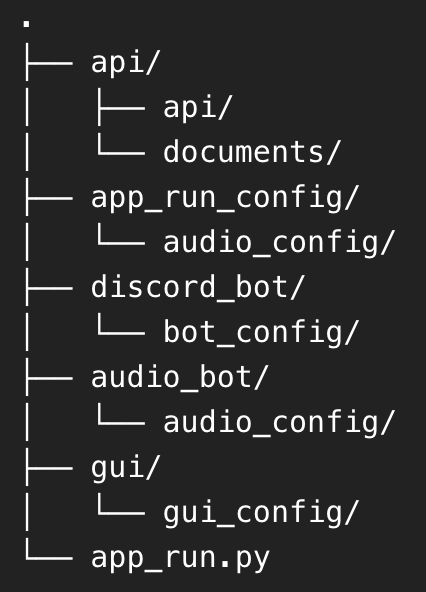
\includegraphics{tree.png}

        \end{center}


	\section{Instrukcja obsługi}
	
		Starting app development
		
			Copy the .env.example file:
			 
		\begin{CPP}
			cp .env.example .env
		\end{CPP}
		
		Modify the environment variables to suit your requirements.
		Launching services
		Install app requirements
		
		\begin{CPP}
			python app_run.py --install
		\end{CPP}
		
		run app
		
		\begin{CPP}
			python app_run.py
		\end{CPP}
		

    \section{Dane wejściowe do działania projektu}

        Jako dane wejściowe projekt potrzebuje nazwy, bądź frazy którą będziemy używać do wywołania komendy, ścieżki lub komendy shell/cmd (w zależności od systemu użytkownika) oraz opcjonalnej dokumentacji na czym polega tworzona komenda.

        \begin{center}

          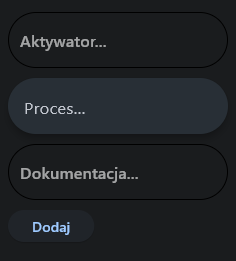
\includegraphics[scale=0.6]{screen3.png}

        \end{center}

    \section{Przykłady działania}

		\subsection{Gui}
        Na początku, zaraz po uruchomieniu programu nie będziemy w stanie od razu wywoływać głosem żadnej komendy, gdyż baza danych jest jeszcze pusta. Aby rozpocząć użytkowanie programu należy dodać komendę, do czego służy pierwszy główny przycisk ``Dodaj komendę''.

        \begin{center}

          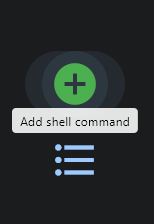
\includegraphics[scale=1.0]{screen2.png}

        \end{center}

        Następnie musimy wpisać odpowiednio opisane już wcześniej interesujące nas parametry oraz kliknąć przycisk ``Dodaj''

        \begin{center}

          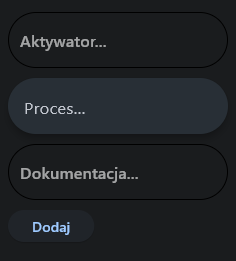
\includegraphics[scale=1.0]{screen3.png}

        \end{center}

        Jeśli jesteśmy tym zainteresowani, możemy ujrzeć listę wszystkich komend, które zostały dodane do bazy danych i możemy wykonywać. Jest to możliwe za pomocą drugiego głównego przycisku ``Wyświetl komendy''.

        \begin{center}

          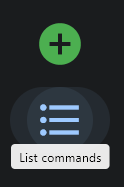
\includegraphics[scale=1.0]{screen4.png}

        \end{center}

        \begin{center}

          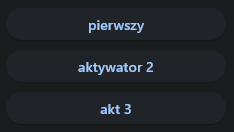
\includegraphics[scale=1.0]{screen5.png}

        \end{center}

        Następnie wystarczy wypowiedzieć słowa wywołujące oraz komendę, którą wcześniej skonfigurowaliśmy.

		\subsection{audio\_bot}
		
		Mikrofon systemowy analizuje mowe i po krótkiej ciszy, wyszukuje podaną frazę w bazie danych, jeśli ją znajdzie, wykona komende przypisaną do tej frazy.
		
		\subsection{discord\_bot}
		
		Użytkownik wpisuje w okienku chatu discorda frazę, po czym jest wyszukiwana w bazie. Przypisana komenda do tej frazy się wykonuje.
		
		\subsection{DoomEmacs}
		
		Użytkownik jest w stanie do bazy dodać komendy elisp, które potrafią zautomatyzować proces programowania, przy uruchomionym emacs serverze.
		
    \section{Podsumowanie}

		Projekt oferuje możliwość zautomatyzowania codziennych czynności i interakcji z zewnętrznymi urządzeniami. 
		
		Wiele dostępnych funkcjonalności jest dopiero bazą, którą można w przyszłości rozwinąć. 
		
        \subsection{Podział pracy w projekcie}

        \begin{itemize}

            \item Rafał Bazan - Team leader, automatyzacja pracy, implementacja Django-ninja API, działalności: PyAudio, discord-bot, DoomEmacs  (backend)
            \item Jakub Piasek - design Graficzny interfejsu Flet, funkcjonalność i implementacja gui, działalności discord-bot (frontend)

        \end{itemize}

    \href{https://github.com/bafaurazan/talk_bot}{Repozytorium na GitHub}

\end{document}
